\startchapter{The StreamIt Language}
\label{chap:language}

This chapter provides an overview and experience report on the basics
of the StreamIt language.  An advanced feature, teleport messaging, is
reserved for Chapter~\ref{chap:messaging}.  For more details on
the StreamIt language, please consult the StreamIt language
specification~\cite{streamit-lang-spec} or the StreamIt
cookbook~\cite{streamit-cookbook}.  A case study on MPEG-2 also
provides excellent examples of the language's
capabilities~\cite{drake-ipdps06}.

\section{Model of Computation}

The model of computation in StreamIt is rooted in (but not equivalent
to) synchronous dataflow~\cite{lee_static_1987}.  As described in
Chapter 1, synchronous dataflow represents a program as a graph of
independent nodes, or {\it actors}, that communicate over FIFO data
channels.  Each actor has an atomic execution step that is called
repeatedly by the runtime system.  The key aspect of synchronous
dataflow, as opposed to other models of computation, is that the
number of items produced and consumed by an actor on each execution is
fixed and known at compile-time.  This allows the compiler to perform
static scheduling and optimization of the stream graph.

StreamIt differs from synchronous dataflow in five respects:
\begin{enumerate}

\item {\it Multiple execution steps.}  Certain pre-defined actors have
  more than one execution step; they are called repeatedly, in a
  cyclic fashion, by the runtime system.  This execution model mirrors
  cyclo-static
  dataflow~\cite{bilsen_cyclo-static_1995,parks_comparison_1995}.  The
  actors that follow this model are {\it splitters} and {\it joiners},
  which scatter and gather data across multiple streams.  (While the
  language once supported multiple execution steps for
  user-programmable actors as well, the benefits did not merit the
  corresponding confusion experienced by programmers.)

\item {\it Dynamic rates.}  The input and output rates of actors may
  optionally be declared to be dynamic.  A dynamic rate represents
  that the actor will produce or consume an unpredictable number of
  data items that is known only at runtime.  Dynamic rates are
  declared as a range (min, max, and a hint at the average), with any
  or all of the elements designated as ``unknown''.  While most of our
  optimizations in StreamIt have focused on groups of static-rate
  actors, we have runtime support for dynamic rates (as demanded by
  applications such as MPEG-2~\cite{drake-ipdps06}).

\item {\it Teleport messaging.}  Our support for irregular,
  out-of-band control messaging falls outside of the traditional
  synchronous dataflow model.  However, it does not impede static
  scheduling.  See Chapter~\ref{chap:messaging} for details.

\item {\it Peeking.}  StreamIt allows actors to ``peek'' at data items
  on their input tapes, reading a value without dequeuing it from the
  channel.  This feature implies that there are two stages to
  scheduling: an initialization schedule that grows buffers until they
  accumulate a threshold number of peeked items, and a steady-state
  schedule that preserves the size of the buffers over time.  While
  peeking can be represented as edge-wise ``delays'' in the original
  nomenclature of synchronous dataflow~\cite{lee_static_1987}, most of
  the scheduling and optimization research on synchronous dataflow
  does not consider the implications of these delays.

\item {\it Communication during initialization.}  StreamIt allows
  actors to input and output a known number of data items during their
  initialization.  This communication is also incorporated into the
  initialization schedule.

\end{enumerate}

With the basic computational model in hand, the rest of this section
describes how StreamIt specifies the computation within actors as well
as the connectivity of the stream graph.

\section{Filters}
\label{sec:filters}

The basic programmable unit in StreamIt is called a {\it filter}.  It
represents a user-defined actor with a single input channel and single
output channel.  Each filter has a private and independent address
space; all communication between filters is via the input and output
channels (and teleport messaging).  Filters are also granted read-only
access to global constants.

An example filter appears in Figure~\ref{fig:fir-streamit}.  It
performs an FIR filter, which is parameterized by a length {\it N}.
Each filter has two stages of execution: initialization and steady
state.  During initialization, the parameters to a filter are resolved
to constants and the {\it init} function is called.  In the case of
FIR, the init function initializes an array of weights, which is
maintained as state within the filter.  During steady state execution,
the {\it work} function is called repeatedly.  Inside of work, filters
can {\it push} items to the output channel, {\it pop} items from the
input channel, or {\it peek} at a given position on the input channel.

\begin{figure}[t]

\begin{minipage}{0.45\textwidth}
\centering
\ninepoint
\begin{verbatim}
float->float filter FIR(int N) {
  float[N] weights;

  init {
    for (int i=0; i<N; i++) {
      weights[i] = calcWeight(i, N);
    }
  }

  work push 1 pop 1 peek N {
    float sum = 0;
    for (int i=0; i<N; i++) {
      sum += weights[i] * peek(i);
    }
    push(sum);
    pop();
  }
}
\end{verbatim}
\end{minipage}
\begin{minipage}{0.55\textwidth}
\centering
\ninepoint
\begin{verbatim}
void init_FIR(float* weights, int N) {
  int i;

  for (i=0; i<N; i++) {
    weights[i] = calc_weight(i, N);
  }
}

void do_FIR(float* weights, int N,
            int* src, int* dest, 
            int* srcIndex, int* destIndex,
            int srcBufferSize, int destBufferSize) {

  float sum = 0.0;
  for (int i = 0; i < N; i++) {
    sum += weights[i] * 
           src[(*srcIndex + i) % srcBufferSize];
  }
  dest[*destIndex] = sum;
  *srcIndex = (*srcIndex + 1) % srcBufferSize;
  *destIndex = (*destIndex + 1) % destBufferSize;
}
\end{verbatim}

%% This version is more parallelizable!
%%
%% /* initialize weights for N-element FIR filter */
%% void init_filter(float* weights, int N) {
%%   int i;
%%  
%%   for (i=0; i<N; i++) {
%%     weights[i] = calc_weight(i, N);
%%   }
%% }
%%
%% /* given weights and an N-element circular buffer,
%%    do filter starting at given position of buffer */
%% float filter(float* weights, float* buffer, 
%%              int pos, int N) {
%%   int i;
%%   float sum = 0;
%%
%%   /* perform weighted sum, starting at index pos */
%%   for (i=0; i<N; i++, pos++) {
%%     sum += weights[i] * buffer[pos];
%%     pos = (pos + 1) % N;
%%   }
%%   return sum;
%% }

\end{minipage}
\begin{minipage}{0.45\textwidth}
\centering
\caption{FIR filter in StreamIt.\protect\label{fig:fir-streamit}}
\end{minipage}
\begin{minipage}{0.55\textwidth}
\centering
\caption{FIR filter in C.\protect\label{fig:fir-c}}
\end{minipage}
\end{figure}

The work function declares how many items it will push and pop, and
the maximum number of items it might peek, as part of its declaration.
To benefit from static scheduling, these expressions must be
resolvable to constants at compile time (dynamic rates are declared
using a different syntax~\cite{streamit-lang-spec}). While a static
analysis can infer the input and output rates in most cases, in
general the problem is undecidable.  Our experience has been that rate
declarations provide valuable documentation on the behavior of the
filter.  In cases where the rates can be inferred, the declarations
can be checked by the compiler.

The StreamIt version of the FIR filter is easy to parallelize and
optimize.  Because there is no mutable state within the filter (that
is, the {\it weights} array is modified only during initialization),
the compiler can exploit data parallelism and instantiate many copies
of the FIR filter, each operating on different sections of the input
tape.  To the best of our knowledge, StreamIt is the first language
that allows tractable parallelization of general-purpose
sliding-window computations such as FIR filters.  Also, due to a lack
of pointers in the language, values can easily be traced through
arrays from their initialization to their use.  This allows the
compiler to infer that the FIR filter computes a linear function,
subject to aggressive optimization~\cite{lamb-pldi03}.  Also,
using a transformation called scalar
replacement~\cite{sermulins:lctes:2005}, the {\it weights} array can
be eliminated completely by unrolling loops and propagating constants
from the init function to the work function.

A traditional C implementation of an FIR filter (shown in
Figure~\ref{fig:fir-c}) resists parallelization and optimization.  The
sliding-window nature of the FIR computation results in a circular
buffer, where elements are addressed using a modulo operation.  Modulo
operations are very difficult to analyze in a compiler; rather than
recognizing the underlying FIFO queue, conservative compilers will
regard each read and write as falling anywhere in an array.  The
problems are confounded by the presence of pointers.  To parallelize
calls to do\_FIR, compilers would need to prove that the {\it weights}
and {\it src} arrays did not overlap with {\it dest}, {\it srcIndex},
or {\it destIndex}.  Similar analysis would be needed to track the
values of {\it weights} from their initialization to their use (in two
different procedures).  Such precise alias analyses are often beyond
reach.  Worse still, it might not even be legal to call {\it do\_FIR}
in parallel, depending on the buffer sizes chosen by the programmer.
The underlying cause of all these obstacles is that the programmer has
over-specified the computation, imposing a scheduling and buffer
management policy that is better decided by the compiler.

Despite its simplicity, this example illustrates the potential of
improving both the programmability and analyzability of stream
programs via a domain-specific language design.  In addition to
exposing the right information to the compiler, the StreamIt version
is also shorter and easier to maintain, representing a win/win
situation for both man and machine.

\begin{figure}[t]
\centering
\begin{minipage}{0.46in}
{\centering
\psfig{figure=pipeline.eps,width=0.46in} \\
}
\end{minipage} 
\hspace{0.15in}
\begin{minipage}{1.3in}
{\centering
\psfig{figure=splitjoin.eps,width=1.3in} \\
}
\end{minipage}
\hspace{0.15in}
\begin{minipage}{1.02in}
{\centering
\psfig{figure=feedback.eps,width=1.02in} \\
}
\end{minipage}
\\ ~ \\ {\mbox{~}\protect\small \mbox{~}(a) A pipeline. ~~~~~(b) A splitjoin. ~~~~~~~~(c) A feedbackloop.~~~~~}
\caption{Hierarchical stream structures in StreamIt.\protect\label{fig:structures}}
\end{figure}

\begin{figure}[t]
\centering
\psfig{figure=fir-pipeline.eps,width=2.33in}
\hspace{0.15in}
\psfig{figure=fir-pipeline2.eps,width=0.46in}
\caption{Example pipeline with FIR filter.\protect\label{fig:pipeline}}
\end{figure}

\begin{figure}[t]
\centering
\psfig{figure=fm-radio-with-code.eps,width=0.9\textwidth}
\caption[Example of a software radio with equalizer]{Example of a
  software radio with equalizer.  There is a natural correspondence
  between the structure of the code and the structure of the graph.
  In the code, stream structures can be lexically nested to provide a
  concise description of the application.\protect\label{fig:fm-radio}}
\end{figure}

\begin{figure}[t]
\centering
\psfig{figure=transpose.eps,width=0.8\textwidth}
\caption{Matrix transpose in StreamIt.\protect\label{fig:transpose}}
\end{figure}

\begin{figure}[t]
\centering
\begin{minipage}{2.5in}
\centering
\psfig{figure=bitreverse-pattern.eps,width=1in}
\end{minipage}
\hspace{0.5in}
\begin{minipage}{3in}
\centering
\psfig{figure=bitreverse-c.eps,width=2.02in}
\end{minipage}

\begin{minipage}{2.5in}
\caption{Data movement in a 3-digit bit-reversed ordering.\protect\label{fig:bitreverse-pattern}}
\end{minipage}
\hspace{0.5in}
\begin{minipage}{3in}
\centering
\caption{Bit-reversed ordering in an imperative language.\protect\label{fig:bitreverse-c}}
\end{minipage}

\end{figure}

\begin{figure}[t]
\centering
\psfig{figure=bitreverse-streamit.eps,width=4.5in}
\caption{Bit-reversed ordering in StreamIt.\protect\label{fig:bitreverse-streamit}}
\end{figure}

\section{Stream Graphs}

One of the new and experimental ideas in StreamIt is to enforce a {\it
  structured} programming model when building stream graphs.  Rather
than allowing programmers to connect filters into arbitrary graphs,
the language provides three hierarchical primitives for building
larger graphs out of smaller ones.  As illustrated in
Figure~\ref{fig:structures}, these structures are a pipeline, a
splitjoin, and a feedbackloop.  Like a filter, each stream structure
has a single input channel and single output channel, allowing them to
be composed and interchanged freely.  We collectively refer to filters
and stream structures as {\it streams}.

The pipeline structure represents a serial composition of streams,
with the output of one stream flowing to the input of the next.
Figure~\ref{fig:pipeline} illustrates the syntax for pipelines; the
{\it add} keyword indicates that a new stream should be instantiated
and appended to the current pipeline.  A splitjoin represents a set of
parallel and independent streams; a {\it splitter} distributes data
from the input channel to the parallel components, while a {\it
  joiner} interleaves the streams' results onto the output channel.
In this case, each call to {\it add} specifies a separate parallel
stream (see Figure~\ref{fig:fm-radio}).  The language provides a fixed
set of pre-defined splitters and joiners, encompassing duplication and
round-robin behavior (more details below).  Finally, the feedbackloop
structure provides a way to induce cycles in the stream graph.

%% The primary motivation for introducing structure in the language is to
%% ensure a disciplined and readable programming style.  There is an
%% analogy here to structured control flow in an imperative language.

The motivations for introducing structured dataflow in a stream
language are analogous to those for introducing structured control
flow in an imperative language.  While there was once a debate between
unstructured control flow (using GOTO statements) and structured
control flow (using if/then/else and for loops), in the end structured
control flow came to dominate because it allows the programmer to
reason locally.  Rather than being lost in a sea of ``spaghetti
code'', programmers can recognize common patterns because the language
forces a canonical and hierarchical expression of the control.  While
skeptics once argued that certain patterns would be more naturally
expressed using GOTO statements, over time there emerged structured
idioms that were equally recognizable.  For example, while a state
machine can be written with GOTO statements for each state transition,
it can also be written as a dispatch loop.  Structured control flow
also benefited compilers, because non-sensical control flow graphs
could be ruled out in favor of the common case.  The entire field of
loop optimizations would have been much more difficult if it had to
address the full complexity of an unstructured programming model.

We believe that imposing structure on a stream graph can offer similar
benefits.  From the programmer's perspective, structured streams offer
a disciplined and readable way to describe, parameterize, and compose
stream graphs.  For example, Figure~\ref{fig:fm-radio} shows the
StreamIt code corresponding to a software radio program.  There are
three things to notice about the figure.  First, there is a natural
correspondence between the structure of the code and the structure of
the stream graph.  Rather than reasoning about an ad-hoc set of nodes
and edges, the programmer can visualize the graph while reading the
code.  Second, the graph description is parameterized.  The number of
parallel streams in the equalizer is dictated by a parameter N.  Thus,
the programmer can easily describe a broad family of stream graphs;
the compiler evaluates the values of the parameters to spatially
unroll the actual stream structure.  Finally, imposing a single-input,
single-output discipline on stream programs enables modularity and
compositionality.  The LowPassFilter and HighPassFilter can be drawn
from a common library, without knowing the details of their internal
representations.

Enforcing structure in the language can also benefit the compiler.
Rather than dealing with the complexity of full graphs, the compiler
can focus on a few simple cases.  This property helped us to formulate
phased scheduling~\cite{karczmarek-lctes03,karczma-thesis} and
linear
optimizations~\cite{lamb-pldi03,lamb-thesis,agrawal-cases05,agrawal-thesis}.
% TODO: revisit later.  Did structure help other things?

We give more details on our experience with structure in Section~\ref{sec:lang-experience}.

\section{Data Reordering}

Another novelty of the StreamIt language is the provision of flexible,
composable, and parameterized language primitives for scattering,
gathering, and reordering data.  These primitives take the form of
pre-defined splitter and joiner nodes, which appear in both splitjoins
and feedbackloops.

There are two types of splitters.  The first splitter, {\it
  duplicate}, copies each input item to all of the output channels.
The second splitter, {\it roundrobin}, is parameterized with a set of
weights, $w_1 \dots w_n$, where $n$ is the number of output channels.
It sends the first $w_1$ input items to the first stream, the next
$w_2$ items to the second stream, and so on, repeating in a cyclic
fashion.  If all of the outputs have the same weight $w$, the splitter
can be written as {\it roundrobin(w)}; similarly, if all the outputs
have weight 1, the programmer can write simply {\it roundrobin}.
Roundrobin is also the only type of joiner available.

By composing these simple primitives -- roundrobin splitters,
roundrobin joiners, and duplicate splitters -- a large number of data
distribution and reordering patterns can be elegantly expressed.  For
example, Figure~\ref{fig:transpose} illustrates StreamIt code for a
matrix transpose.  The reordering needed can be expressed by a single
splitjoin.  The splitjoin has an empty stream for every column in the
matrix; a roundrobin(1) splitter moves the columns into the splitjoin,
while a roundrobin(M) joiner moves the rows to the output channel.

Another example is bit-reversed ordering.  As illustrated in
Figure~\ref{fig:bitreverse-pattern}, a bit-reversed ordering is a
permutation in which the element at index $n$, where $n$ has binary
digits $b_0b_1 \dots b_k$, is reordered to appear at index $b_kb_{k-1}
\dots b_0$.  For example, in a 3-digit bit reversal, the item at index
one (001) is reordered to index four (100).  In a traditional language
such as C, the code to perform bit-reversal is very complex; see
Figure~\ref{fig:bitreverse-c} for a standard
algorithm~\cite{press_numerical_1992}.  Given the doubly-nested loops,
conditionals, shift expressions, and swap operations, it is unlikely
that any compiler will arrive at a sensical representation for the
logical reordering performed by this computation.  It is equally
difficult for humans to comprehend the code.

However, the StreamIt version (Figure~\ref{fig:bitreverse-streamit})
of bit reversal is far simpler~\footnote{Satish Ramaswamy in our group
  discovered this representation of bit-reversal.}.  It represents bit
reversal as a recursive reordering.  In the base case, there are only
two elements and no reordering is needed (a 1-digit bit reversal is
the identity operation).  Otherwise, the reordering consists of
separating elements into two groups based on the lowest-order bit of
the input position, reordering both groups independently, and then
joining the groups based on the highest-order bit of the output
position.  This pattern can be expressed with a roundrobin(1)
splitter, a recursive call to BitReverse(N/2), and a roundrobin(N/2)
joiner.  The intuition is: bit reversal is equivalent to a tree of
fine-grained splitting and coarse-grained joining.  A graphical
depiction of this tree also appears in
Figure~\ref{fig:bitreverse-streamit}.

Why bother to represent distribution and reordering operations in an
elegant and analyzable way?  The reason is that stream programming
centers on data movement, and preserving information about exactly
where each data item is going enables the compiler to perform more
aggressive optimizations.  For example, standardized splitters and
joiners have enabled us to map reordering operations to a programmable
on-chip network~\cite{streamit-asplos} and have enabled certain
domain-specific
optimizations~\cite{lamb-pldi03,agrawal-cases05,techreport}.
Other researchers have also leveraged this representation to
automatically generate vector permutation
instructions~\cite{mani-permutations} and to facilitate program
sketching~\cite{bit-streaming}.

While the reordering primitives we have defined are quite expressive,
it should be noted that they are not complete.  Because splitters
always distribute their first input item to the first output channel
(and likewise with joiners), it is impossible to express a pure
permutation in which the first item is reordered to a different
position of the stream.  However, this behavior can be emulated by
introducing simple computational nodes, such as a filter that
decimates some of its inputs.  Of course, it could also be rectified
by adding programming language support for adjusting the order of
items output.  We have not found this functionality to be needed in
our application set.

%% Some programs are elegant, some are exquisite, some are sparkling.
%% My claim is that it is possible to write grand programs, noble
%% programs, truly magnificient ones!
%% -- Don Knuth, Computer Programming as an Art, ACM Turing Award Lecture, 1974

\section{Experience Report}
\label{sec:lang-experience}

\begin{table}[t]
\centering
%% - streamit benchmark suite
%%   - table:
%%     - benchmark name
%%     - benchmark description / reference
%%     - number of static / dynamic streams
%%     - number peeking
%%     - number stateless?
%%       - better: fraction of stateful work, largest work in stateful filter
%%     - number of messaging pairs
%%     - parameterized by -- how the benchmark can grow
%%     - number of splitjoins, feedback loops
%%     - author(s)
%%     - lines of code
%%     - dynamic control flow?
{\small
\begin{verbatim}
Ground Moving Target Indicator (GMTI)      GSM decoder                       
Feature-Aided Tracker (FAT)                FM software radio                 
Synthetic Aperture Radar (SAR)             DES and serpent encryption        
Radar array front-end                      Matrix multiplication             
3GPP physical layer subset                 Graphics shading and rendering    
Vocoder with speech transformation         Sample rate converter             
MP3 decoder subset                         Target detector                   
MPEG-2 encoder and decoder                 Channel vocoder                   
MPEG-4 decoder subset                      Library of DCTs, FFTs, Filterbanks
JPEG encoder and decoder                   Library of sorting algorithms     
\end{verbatim}}
%TODO: include detailed application characteristics, possibly stream graphs
\caption{StreamIt benchmark suite.\protect\label{tab:lang-benchmarks}}
\end{table}

%% TODO: add all the stream graphs?
%% could be annotated with:
%% - amount of work
%% - stateful / stateless
%% - dynamic control flow
%% - peeking
%% - I/O rates

The StreamIt benchmark suite is detailed in
Table~\ref{tab:lang-benchmarks}.  In addition to our own benchmarks,
researchers at Halmstad University have used StreamIt to develop a
medium pulse repetition frequency doppler radar
(MPD)~\cite{ola-techrep}.  The largest benchmarks are GMTI, MPEG-2,
FAT, and SAR.  At the time of this writing, shortcomings in the
compiler have prevented us from obtaining performance numbers for
these complete applications.  However, their functional correctness
has been verified in the Java runtime for the StreamIt language.

While our initial conception of stream programs proved to be generally
accurate, in developing the benchmark suite we encountered a few
surprises regarding the benchmarks' common-case behavior.  The
following observations should be taken in the context of our own
benchmark suite, which is necessarily limited and biased.  However,
they might nonetheless be informative for other researchers:

\begin{enumerate}

\item {\it Filters rarely contain mutable state.}  While other
  researchers have noted that stream programs are rich in data
  parallelism~\cite{imagine03ieee}, we nonetheless expected to see a
  greater proportion of filters that retained mutable state between
  execution steps.  Without mutable state, filters can be split into
  multiple instances that operate on separate sections of the input
  stream; this is perhaps the most straightforward parallelism to
  exploit.  However, with mutable state, only one instance of the
  filter is possible, and the compiler must exploit task- and
  pipeline-parallelism between the filter and others in the graph.

  The state observed can be explained as follows.  Vocoder performs an
  adaptive DFT that uses a stateful decay to ensure stability; it also
  needs to retain the previous output across one iteration within a
  phase transformation.  MPEGDecoder maintains significant state in
  the parser, and also has negligible state in retaining predicted
  motion vectors across one iteration of work.  Radar repeatedly
  operates on long columns of an array requiring special behavior at
  the boundaries; thus, the state tracks the position in the column
  and does some internal buffering.  Radar can be rewritten at a
  coarse level of granularity to eliminate this state.

  We are currently expanding our benchmark suite to explore more
  stateful applications, including intelligent network routing (which
  maintains per-flow state) as well as cache simulation (in which the
  simulated memories represent state).

\item {\it Neighboring filters often have matched I/O rates.}  Many of
  the advanced scheduling strategies for synchronous dataflow graphs
  have the highest payoff when the input and output rates of
  neighboring filters are mismatched.  For example, the CD-DAT
  benchmark (shown in Figure~\ref{fig:cd-dat}) is used in many
  studies~\cite{murthy_minimizing_1994,bhattacharyya_optimal_1995,teich_3d_1999,bhattacharya_quasi-static_2000,chandrachoodan_efficient_2001,murthy_buffer_2004,ko_memory-constrained_2006};
% TODO: this was first page of google results for unquoted string, ``cd-dat dataflow''
%  - fill in the rest
  it converts compact disk auto (sampled at 44.1 khz) to digital audio
  tape (sampled at 48 khz).  Performing this conversion in stages
  improves efficiency~\cite{murthy_minimizing_1994}.  However,
  neighboring filters have different communication rates which share
  no common factors, resulting in a large steady-state schedule.

  In our benchmark suite, mismatched communication rates as seen in
  CD-DAT are very rare.  The common case is that the entire benchmark
  is operating on a logical frame of data which is passed through the
  entire application (such as in FFT, see Figure~\ref{fig:fft}).
  Sometimes there are difference in the input and output rates for
  filters that operate at different levels of granularity; for
  example, processing one frame at a time, one macroblock at a time,
  or one pixel at a time.  However, these rates have a small common
  multiple (i.e., the frame size) and can be accommodated without
  growing the steady state schedule.

  The most quantitative evidence that we have to this effect is
  detailed in our paper on phased
  scheduling~\cite{karczmarek-lctes03}.  The paper develops a new
  scheduling algorithm that reduces the buffer requirements needed to
  execute a synchronous dataflow graph.  The space saved on CD-DAT is
  over 14x.  However, the median savings across our entire benchmark
  suite is less than 1.2x.  The reason is that the potential savings
  on most benchmarks was extremely small due to matched input and
  output rates; simply executing each node once would often give the
  minimal possible buffering.

\begin{figure}[t]
\centering
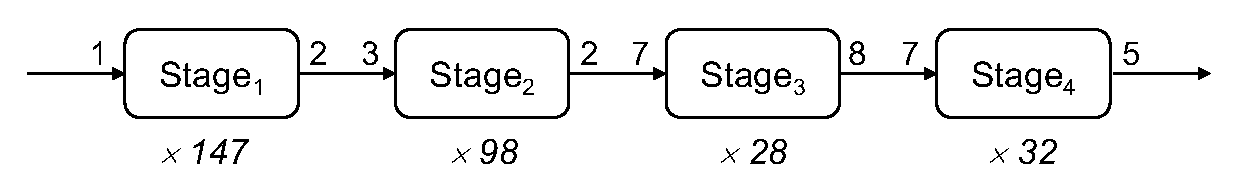
\psfig{file=cd-dat,width=4.5in}
\caption[CD-DAT, an example of mismatched I/O rates]{The CD-DAT
  benchmark~\cite{murthy_buffer_2004} exhibits unusually mis-matched
  I/O rates.  Nodes are annotated with the number of items pushed and
  popped per execution, as well as their execution multiplicity in the
  steady state. Since neighboring filters produce different numbers of
  items, each filter has a large multiplicity in the steady state.
  This demands clever scheduling strategies to avoid extremely large
  buffer sizes.\protect\label{fig:cd-dat}}

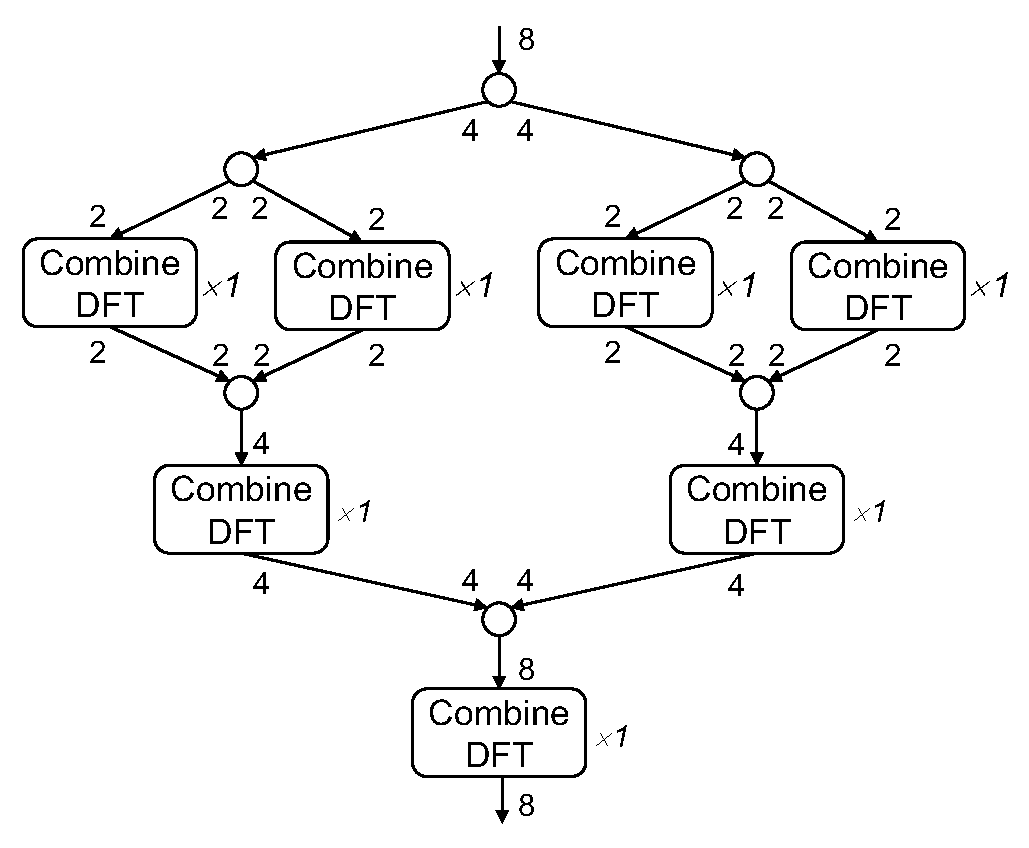
\psfig{file=fft.eps,width=4in}
\caption[FFT, an example of matched I/O rates]{The FFT benchmark, like
  many benchmarks, exhibits matched I/O rates.  Nodes are annotated
  with the number of items pushed and popped per execution, as well as
  their execution multiplicity in the steady state.  Since neighboring
  filters produce the same number of items on each execution, each
  filter executes only once in the steady state.  This provides less
  flexibility and benefit for optimizing the
  schedule.\protect\label{fig:fft}}

\end{figure}

\item {\it There are few feedback loops in our benchmarks.}  While we
  did not intend to focus on acyclic programs, the benchmarks we
  encountered were often free of feedback loops.  Notable exceptions
  are MPEG-2 encoding and mosaic imaging, which both contain irregular
  feedback loops that are implemented using teleport messaging.
  messaging.

\end{enumerate}

In addition to our observations about the benchmark characteristics,
we also offer some lessons learned from developers' experiences in
implementing stream programs.  As noted in
Table~\ref{tab:lang-benchmarks}, the StreamIt benchmarks were
developed by many different people, mostly undergraduates at MIT.  As
the developers were newcomers to the StreamIt language, we expect that
their experience would reflect that of a broader user population;
their coding style was not influenced by the intent of the original
language designers.  We summarize their experience as follows:

\begin{enumerate}

\item {\it Structured streams are a useful and tractable means of
  writing programs.  However, they are occasionally unnatural and, in
  rare cases, insufficient.}  Overall, we found structured streams --
  the hierarchical composition of pipelines, splitjoins, and
  feedbackloops -- to be a good match for the applications in our
  benchmark suite.  While the developer sometimes had to refactor an
  unstructured block diagram into structured components, the result
  was nonetheless a viable way to represent the application.

\begin{figure}[t]
\centering
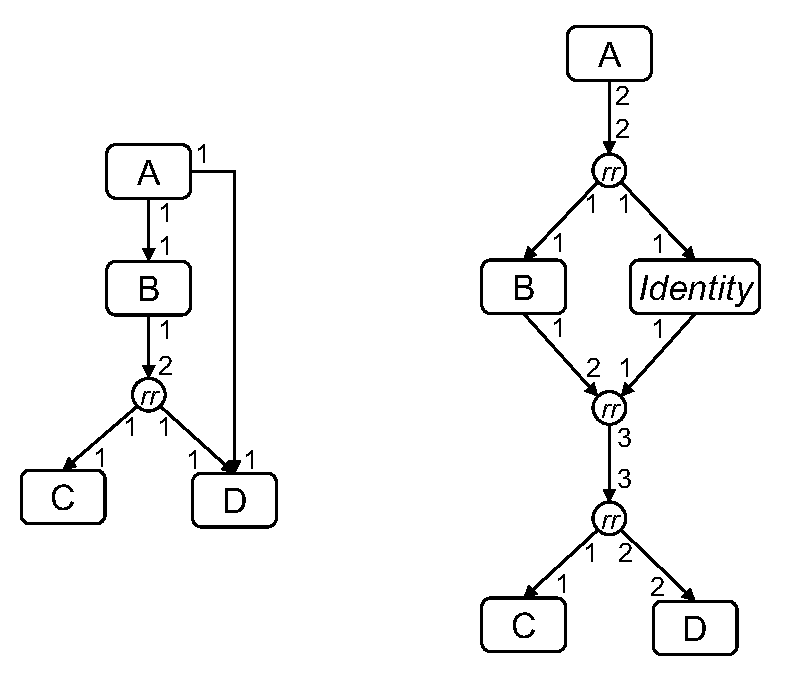
\psfig{file=interleaving.eps,width=3.5in}

(a) Unstructured ~~~~~~~~~~~~~~~~~~~~~~~~~ (b) Structured~~~~~~
\caption[Refactoring a stream graph to fit a structured programming
  model]{Example of refactoring a stream graph to fit a structured
  programming model.  Both graphs achieve equivalent communication
  between filters.
\protect\label{fig:interleaving}}
\end{figure}

  One shortcoming of structure is that it can force programmers to
  multiplex and demultiplex conceptually-distinct data streams into a
  single channel.  The underlying cause of this hazard is illustrated
  in Figure~\ref{fig:interleaving}.  Because filters C and D are
  running in parallel, their input streams must converge at a common
  splitter under a structured programming model.  However, this
  implies that the auxiliary communication from A to D must also pass
  through the splitter, in a manner that is interleaved with the
  output of B.  An extra splitjoin (at the top of
  Figure~\ref{fig:interleaving}b) is needed to perform this
  interleaving.  A more realistic example of the same hazard is shown
  in Figure~\ref{fig:3gpp}, which is taken from our 3GPP benchmark.

  Needless to say, this pattern of multiplexing and demultiplexing
  adds considerable complexity to the development process.  It
  requires the programmer to maintain an unwritten contract regarding
  the logical interleaving of data streams on each physical channel.
  Moreover, the addition of a new communication edge in the stream
  graph may require modification to many intermediate stages.

  While there is no perfect solution to this problem, we have
  sometimes embraced two imperfect workarounds.  First, the data items
  in the multiplexed streams can be changed from a primitive type to a
  structure type, allowing each logical stream to carry its own name.
  This approach would benefit from a new kind of splitter and joiner
  which automatically packages and un-packages structures from
  adjoining data channels.  The second approach is to employ teleport
  messaging; as described in the next chapter, it allows
  point-to-point communication and avoids interleaving stream data.
  However, since it is designed for irregular control messages, it
  does not expose information about the steady-state dataflow to the
  compiler.

  In practice, we have chosen to tolerate the occasional complexity of
  stream multiplexing rather than to fall back on an unstructured
  programming model.  However, it may be valuable to consider a
  natural syntax for unstructured components of the stream graph --
  the analog of break and continue statements (or even a rare GOTO
  statement) in structured control flow. It is important to note,
  however, that there is no overhead introduced by adding splitters
  and joiners to the stream graph; the StreamIt compiler analyzes the
  communication (via an analysis known as {\it synchronization
  removal}) to recover the original unstructured communication.

\begin{figure}[t!]
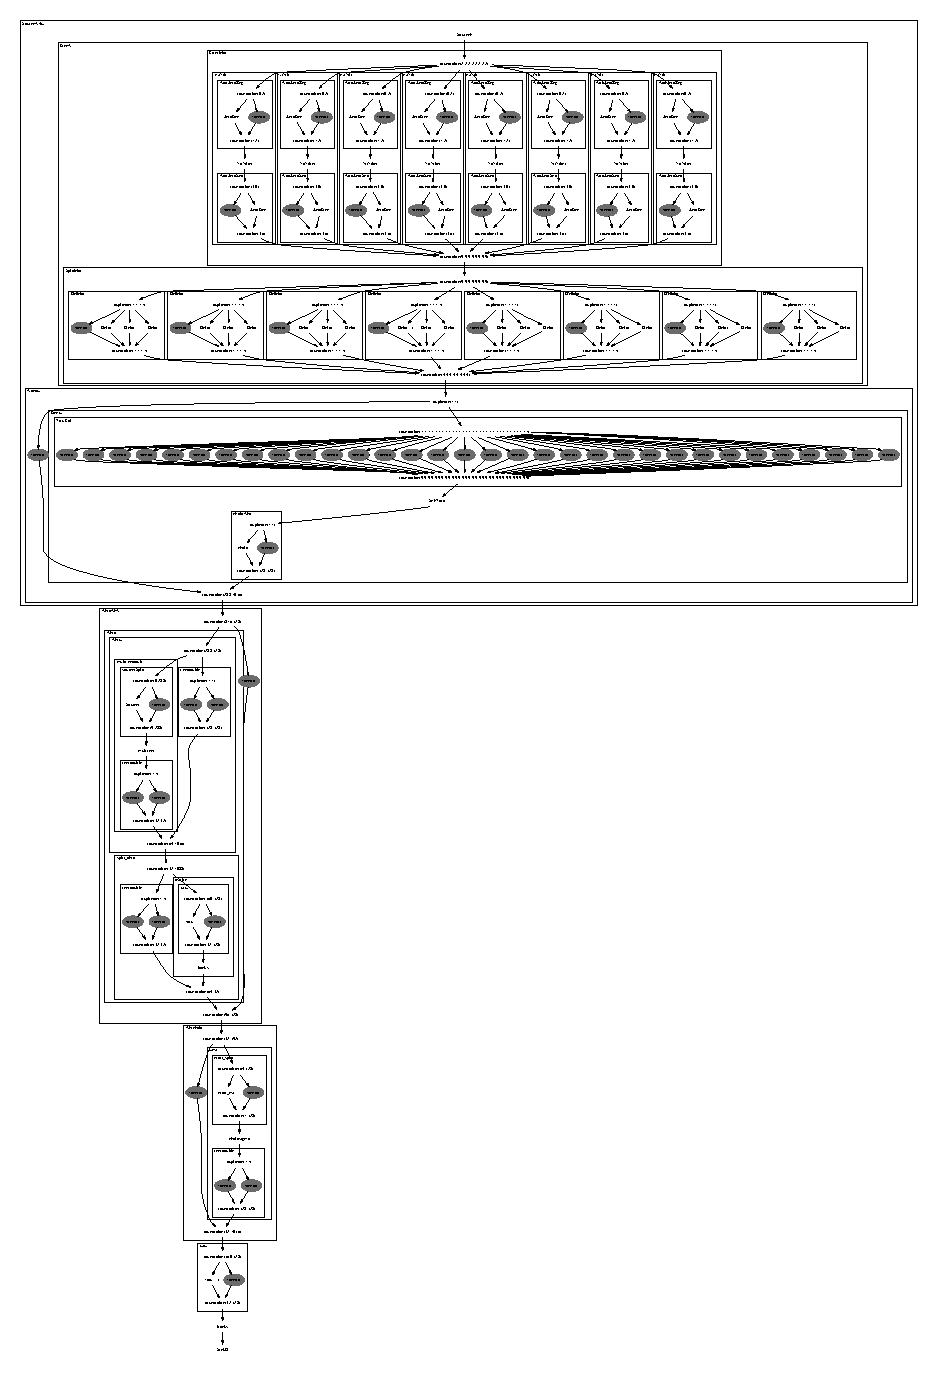
\psfig{file=3gpp.eps,height=\textheight}
\vspace{-1.25in} ~ \\
\begin{minipage}{4in}
\caption[Stream graph for 3GPP]{Stream graph a 3GPP Radio Access
  Protocol application.  Shaded filters indicate Identity nodes that
  are used to bypass data items around intermediate filters.  They are
  also used in splitjoins for data duplication and
  reordering.\protect\label{fig:3gpp}}
\end{minipage}
\end{figure}

\begin{figure}[t]
\centering
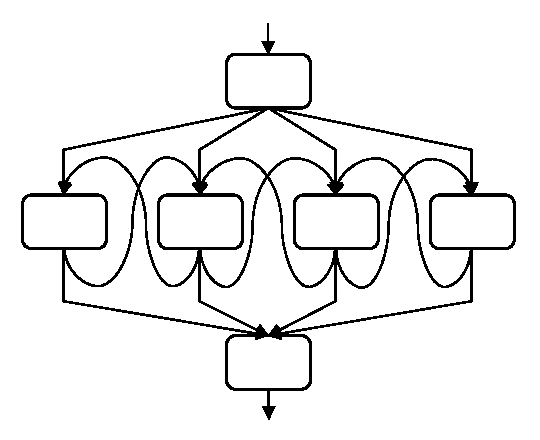
\psfig{file=inadequate.eps,width=2in}

\caption[A communication pattern unsuitable for structured streams.]{A
  communication pattern unsuitable for structured streams.  This
  pattern can arise in video compression, where each block informs its
  neighbors of its motion prediction before the next processing
  step.\protect\label{fig:inadequate}}.
\end{figure}

  Finally, there are rare cases in which the structured primitives in
  StreamIt have been inadequate for representing a streaming
  communication pattern.  Figure~\ref{fig:inadequate} illustrates an
  example from video compression, where each parallel filter performs
  a motion prediction for a fixed area of the screen.  Between
  successive frames, each filters shares its prediction with its
  neighbors on either side.  While this could be represented with a
  feedback loop around the entire computation, there would be
  complicated interleaving involved.  This case reflects a broader
  shortcoming, discussed below, that StreamIt is not designed for
  multidimensional data processing.

\item {\it Programmers can accidentally introduce unnecessary mutable
  state in filters.}  Filters that have no mutable state are
  attractive because they can be run in a data-parallel fashion.
  Unfortunately, the performance cost of introducing state is not
  exposed in the current StreamIt language.  Thus, we found that
  several programmers, when faced with two alternative implementations
  of an algorithm, would sometimes choose the one that included
  mutable state (see Figure~\ref{fig:state} for an example).  Prior to
  conducting our performance evaluations, we examined all stateful
  filters in the benchmarks and rewrote them as stateless filters when
  it was natural to do so.  In a future stream languages, it may be
  desirable to require an extra type modifier on stateful filters,
  such as a {\it stateful} keyword in their declaration, to force
  programmers to be cognizant of any added state and to avoid it when
  possible.

\begin{figure}[t]
\hspace{0.1\textwidth}
\begin{minipage}{0.35\textwidth}
\centering
\ninepoint
\begin{verbatim}
void->int filter SquareWave() {
  work push 2 {
    push(0);
    push(1);
  }
}
\end{verbatim}
\end{minipage}
\hspace{0.1\textwidth}
\begin{minipage}{0.35\textwidth}
\centering
\ninepoint
\begin{verbatim}
void->int filter SquareWave() {
  int x = 0;
 
  work push 1 {
    push(x);
    x = 1 - x;
  }
}
\end{verbatim}
\end{minipage}

\hspace{0.1\textwidth}
\begin{minipage}{0.35\textwidth}
\centering
(a) Stateless
\end{minipage}
\hspace{0.1\textwidth}
\begin{minipage}{0.35\textwidth}
\centering
(b) Stateful
\end{minipage}
\caption[Accidental introduction of filter state]{Programmers can
  accidentally introduce unnecessary filter state when writing
  programs.  In this example, the intended output is a square wave,
  emitting alternate values of 0 and 1.  Both implementations shown
  are functionally equivalent.  However, the stateless version (a)
  appears data-parallel to the compiler, while the stateful version
  (b) appears sequential.\protect\label{fig:state}}
\end{figure}

\item {\it Multi-phase filters confuse programmers and are not
  necessary.}  At one point in the StreamIt project, we embraced the
  cyclo-static dataflow
  model~\cite{bilsen_cyclo-static_1995,parks_comparison_1995} for all
  filters.  Under this model, the programmer can define multiple work
  functions that are executed under a specified pattern.  By dividing
  execution into more fine-grained units, cyclo-static dataflow can
  offer lower latency than synchronous dataflow, and can also avoid
  deadlock in tightly constrained loops.

  However, our experience is that having the option of multiple
  execution steps is confusing to beginning StreamIt programmers.
  There is a tendency to interpret multiple execution steps as
  belonging to multiple distinct filters.  It is also difficult to
  explain to a non-expert why one method should be designated as an
  execution step, rather than as a plain subroutine call.

  Multiple execution steps did prove to be important to the semantics
  of splitters and joiners, which would have an unreasonably large
  granularity if they were forced to transfer a full cycle of data at
  a single time.  However, because StreamIt relies on a few built-in
  primitives for splitting and joining, the subtlety of this execution
  semantics could be hidden from the programmer.  Apart from splitters
  and joiners, we did not encounter any scenarios (in our limited
  benchmark suite) that demanded multiple execution steps in filters.

  Thus, after making a significant investment to support the full
  generality of cyclo-static dataflow in the StreamIt compiler, we
  eventually changed course and removed the capability from the
  language.

\item {\it Input and output rates can typically be inferred from the
  code inside a filter.  However, it is still worthwhile for the
  programmer to declare them.}  We were surprised how many StreamIt
  benchmarks contained completely static control flow inside the body
  of filters.  That is, the path of control taken through the {\it
    work} function is often independent of the data values input to
  the filter.  Exceptions to this pattern include sorting algorithms,
  compression algorithms, and parsing algorithms (e.g., the MPEG-2
  bitstream parser).

  When the control flow is static, it is often feasible for the
  compiler to infer the number of items pushed and popped via a static
  analysis.  Such an analysis could save the programmer the trouble of
  annotating each work function with its input and output rates.

  However, we did find that it is valuable for programmers to annotate
  the input and output rates even when they can be inferred.  As is
  commonly the case with type declarations, these annotations provided
  documentation to other users regarding the intended behavior of the
  filter, making it easier to understand and maintain.  They also
  provided a level of redundancy, so that, when possible, the compiler
  could check the consistency between the declared rates and the
  actual implementation.

\end{enumerate}

\section{Related Work}
\label{sec:lang-related}

As described in Chapter 1 and elsewhere~\cite{stephens_survey_1997}, there is a
long history of programming language support for streams in the
dataflow, functional, and synchronous language domains.  Here we
compare to StreamIt's more immediate contemporaries.

The Brook language is architecture-independent and focuses on data
parallelism~\cite{brook04}.  Stream kernels are required to be
stateless, though there is special support for reducing streams to a
single value.  Stream\-C/Ker\-nel\-C is lower level than Brook;
kernels written in KernelC are stitched together in StreamC and mapped
to the data-parallel Imagine processor~\cite{imagine03ieee}.  SPUR
adopts a similar decomposition between ``microcode'' stream kernels
and skeleton programs to expose data parallelism~\cite{spur05samos}.
Cg exploits pipeline parallelism and data parallelism, though the
programmer must write algorithms to exactly match the two pipeline
stages of a graphics processor~\cite{cg03}.  Compared to these
languages, StreamIt places more emphasis on exposing task and pipeline
parallelism (all the languages expose data parallelism).
%and on sliding window operations (filters that peek).  
By adopting the synchronous dataflow model of execution, StreamIt
focuses on well-structured and long-running programs that can be
aggressively optimized.  We are not aware of structured streams or
hierarchical mechanisms for data reordering in other stream languages.
%The implicit infinite loop around programs is
%also a key StreamIt characteristic that enables optimizations.
Spidle~\cite{spidle03} is also a recent stream language that was
influenced by StreamIt.

\section{Future Work}

There are many directions in which to expand and refine the StreamIt
language.  Based on his study of MPEG-2 in StreamIt, Matthew Drake
makes a sound case for adding support for programmable splitters and
joiners, re-initialization of streams, draining of streams, and
dispatch splitjoins~\cite{drake-thesis}.  He also discusses extensions
to messaging, discussed in the next chapter.  We endorse his
recommendations and also highlight the following research directions:

% cite written proposal to move programmable splitters and joiners
% into the language?

\begin{enumerate}

\item {\it Dynamic changes to stream structure.}  A long-time goal of
  the StreamIt group has been to define and implement support for
  dynamic changes to the stream graph.  For example, an adaptive
  channel decoder may decide to add or remove filtering stages; an FIR
  filter may dynamically scale the size of the window it considers; a
  network router may add or remove streams to represent new logical
  flows; or an AMPS cellular base station may add and remove streams
  to support new clients.

  There are several challenges and opportunities in supporting dynamic
  stream graphs.  As described in the next chapter, our basic model
  for runtime adaptation is to re-evaluate the initialization code for
  stream structures by sending a teleport message to that stream.  The
  difficulty comes in timing the re-initialization, defining the
  transition between graphs, and maintaining as much static
  information as possible about the possible configurations of graphs
  that will be adopted at runtime.  While we have developed extensive
  internal notes and proposals on language support for dynamism, we
  omit them from this dissertation because we have yet to reach
  consensus on many aspects of the design.

  As an intermediate step towards supporting a fully-reconfigurable
  stream graph, it would also be interesting to introduce primitives
  that allow programmers to indicate which parts of code should be
  evaluated at compile time, versus being evaluated at load time or
  runtime.  The current StreamIt compiler requires the structure and
  communication rates in the stream graph to be evaluated at compile
  time, though the StreamIt language could also be interpreted as
  binding these values at load time (during program initialization).
  While compile-time evaluation improves optimization opportunities,
  it is not always permissible by the application.  For example, if an
  external file is used to drive the structure or parameters of the
  stream graph, then compile-time evaluation is safe if that file is
  fixed across all executions (e.g., a simulator for a specific
  processor architecture) but unsafe if it may vary from one execution
  to the next (e.g., a scene description for a rendering engine).  We
  envision that a simple type modifier, such as a ``dynamic'' keyword,
  could be used to distinguish these cases.  The type system would
  guarantee that everything that depends on dynamic data is also
  declared dynamic.  This would allow the compiler to maximally
  evaluate other sections of the stream graph at compile time.

\item {\it Multidimensional data.}  The current version of StreamIt is
  a natural fit for handling one-dimensional sequences of data, but
  falls short in exposing the dependences and flexibility inherent in
  manipulating multi-dimensional data.  When handling sequences of
  multidimensional data (such as video frames), the programmer is
  currently left with two alternatives.  One option is to take a
  coarse-grained approach in which filters push and pop entire arrays
  at a time.  However, this results in nested loops within filter
  code, reducing the problem to a traditional loop analysis without
  gaining any leverage from the streaming domain.  The second option
  is to take a fine-grained approach, in which individual arrays are
  split up into columns or blocks and distributed over many filters.
  However, this mapping forces the programmer to specify a fixed
  decomposition of the data in the array (row-major, column-major,
  blocked, etc.) and makes it more difficult for the compiler to infer
  the underlying dependences and adjust the schedule as needed.

  One possibility for handling multidimensional data could be to add
  iterators that apply a filter (or entire stream graph) to all of the
  elements of an array.  The Brook language~\cite{brook04} adopts a
  similar approach in a construct termed {\it stencils}.  However,
  stencils generally operate on a single array at a time and are not
  integrated into a larger stream graph.  An opportunity for future
  work would be to create a unified environment for processing
  sequences of arrays and data items within arrays, including
  compiler-friendly ``bridge'' operators that decompose arrays into
  data streams and assemble data streams into arrays.  Research
  challenges arise in the specification of boundary conditions on the
  sides of an array, the dependences and reuse between different parts
  of an array, and the possibility for carried state across separate
  arrays.

\item {\it External interfaces.}  In practice, it is important for any
  domain-specific language to have well-defined interfaces for
  interacting with languages and systems that fall outside of the
  domain.  In the case of streaming, this encompasses interfaces for
  embedding stream graphs within general purpose languages, as well as
  for embedding general-purpose computations within stream graphs.
  While we have developed an internal, ad-hoc interface for
  interfacing between StreamIt and C, there are interesting research
  questions in rigorously defining the semantics of such hybrid
  computational models. 

  For example, one characteristic of synchronous dataflow is that data
  streams are virtually infinite; however, from a general-purpose
  language, streaming computations can also be gainfully applied to
  large arrays.  Thus, it will be valuable to develop formal notions
  of draining the stream graph, and perhaps mechanisms to maintain the
  state of a stream graph from one instantiation to another.

  There are also interesting questions that relate to the memory model
  of hybrid systems.  Synchronous dataflow represents a fully
  distributed model with no access to shared state; however, other
  general-purpose programming models often embrace a shared-memory
  abstraction.  As described in the next chapter, one approach to
  unifying these abstractions could be to allow streaming updates to
  shared memory so long as they are committed according to a
  deterministic static schedule.

\end{enumerate}

\section{Chapter Summary}

This chapter describes the design rationale and experienced gained
from the StreamIt language, one of the first programming languages
that exposes and exploits the inherent regularity of stream programs.
StreamIt is rooted in the synchronous dataflow model, with added
support for multiple execution steps, dynamic communication rates,
teleport messaging, peeking, and communication during initialization.
Key novelties of the language are the notion of structured streams,
akin to structured control flow in an imperative language, as well as
hierarchical and parameterized splitjoins for data reordering.  The
design of the basic computational node in StreamIt, the filter, also
exposes inherent parallelism that is masked by pointer manipulation
and modulo operations in a traditional C implementation.

The development of a large-scale benchmark suite in StreamIt led to
several insights and surprises.  In our benchmarks, we were surprised
how few filters contained mutable state; this suggests that many
programs can leverage data parallelism, rather than relying on task
and pipeline parallelism, to achieve parallel performance.  Our
benchmarks often contain matched input and output rates, where filters
need to execute only a small number of times before satisfying the
steady-state data requirements of their neighbors.  This property
reduces the space of scheduling alternatives as well as the benefit
derived (e.g., in buffer space) from complex filter interleavings.
Our benchmark suite also contained few feedback loops.  Of course,
these observations are valid only insofar as our choice of benchmarks;
we are actively expanding our coverage to include other styles of
programs that may lead to different conclusions.

Continuous feedback from StreamIt developers also provided a valuable
critique of the StreamIt language.  While structured streams were a
natural way to represent common programs, in some cases the programmer
needed to refactor an unstructured stream graph into a more complex
structured representation.  An optional mechanism for infrequent
unstructured communication may be valuable in future languages.
Programmers were also prone to accidentally introduce mutable filter
state, impeding parallelization.  Future languages should expose this
performance cost to the programmer so that they avoid unnecessary
serialization.  We found that multi-phase filters (as in cyclo-static
dataflow) are likely to confuse programmers and are not necessary to
express computations in our benchmark suite.  Finally, while the input
and output rates of most filters could be inferred, it was still
worthwhile to declare them from a software engineering standpoint.

There is rich potential for future work in stream languages, including
support for dynamically changing the stream structure, support for
multidimensional data, and support for external interfaces.
